\section{Display management}
\label{dispmanagement}
Oberon's display system comprises 2 main topics:
\begin{enumerate}
  \item \emph{viewer management} (VM), and
  \item \emph{cursor handling}.
\end{enumerate}
Let us 1st turn to the much more involved topic of 1 and postpone 2 to the end of this section.
Before we can actually begin our explanations
we need to introduce the concept of the \emph{logical display area}.
It is modeled as a 2-dimensional Cartesian plane
housing the totality of objects to be displayed.
The essential point of this abstraction is a rigorous decoupling
of any aspects of physical display devices.  As a matter of fact,
any concrete assignment of display monitors to certain finite regions of the display area
is a pure matter of configuring the system.

Being a subsystem of OS with well-defined modular structure,
the display system appears in the form of a small hierarchy of modules.
Its core is a linearly ordered set consisting of 3 modules:
\begin{table}[h!]
  \centering
  \begin{tabular}{l}
    \verb|Display|, \\
    \verb|Viewer|s, and \\
    \verb|MenuViewer|s,
  \end{tabular}
\end{table}
\\the latter building upon the former.  Conceptually, each module contributes
an associated class of display-oriented objects and a collection of related service routines.

The following is an overview of the subsystem VM.
\begin{table}[h!]
  \setlength{\tabcolsep}{2pt}
  \begin{tabular}{l|l|l}
    Module     &Type   &Service \\\hline
    MenuViewer &Viewer &Message handling for menu viewers \\
    Viewers    &Viewer &Tiling VM \\
    Display    &Frame  &Block-oriented raster operations
  \end{tabular}
\end{table}
\begin{table}[h!]
  \setlength{\tabcolsep}{2pt}
  \begin{tabular}{r l l}
    Modules&on upper lines&import lower ones, and \\
      types&on upper lines&extend those on lower.
  \end{tabular}
\end{table}

Inspecting the "Type" column we recognize precisely our familiar types
\begin{table}[h!]
  \centering
  \begin{tabular}{l}
    \verb|Frame|, \\
    \verb|Viewer|, and \\
    \verb|MenuViewer| respectively,
  \end{tabular}
\end{table}
\\where the last is an abbreviation of \verb|MenuViewers.Viewer|.
\\In addition to the core modules of the display system
a section in \verb|Oberon| provides a specialized API that simplifies the use of the VM package
by applications in the case of standard Oberon display configurations.
We shall come back to this topic in \textsection \ref{sec:stdispconf}.

For this moment let us concentrate on the VM core and in particular the \verb|Viewer|s
and \verb|MenuViewer|s, saving the \verb|Display| for the next section.
Typically, we start a module presentation by listing and commenting its definition,
and refer to subsequent listings for its implementation.

\subsection{Viewers}
Focusing 1st on module \verb|Viewer|s we can roughly define the domain of its responsibility as
\emph{initializing and maintaining the global layout of the display area}.  From the previous discussion
we are well acquainted already with the structure of the global display space as well as its building blocks:
\begin{quote}
The display area is hierarchically tiled with frames, where the first two levels
in the frame hierarchy correspond to \emph{tracks} and \emph{viewers} respectively.
\end{quote}
The formal definition:
\begin{verbatim}
DEFINITION Viewers;
  IMPORT Display;              (*message ids*)
  CONST restore = 0; modify  = 1; suspend = 2;
  TYPE Viewer = POINTER TO ViewerDesc;
       ViewerDesc = RECORD (Display.FrameDesc)
                           state: INT  END;
       ViewerMsg = RECORD (Display.FrameMsg)
                          id, X, Y, W, H: INT;
                          state: INT  END;
  VAR curW: INT; (*currently configured width*)

  PROC InitTrack(W, H: INT; Filler: Viewer);
  PROC OpenTrack(X, W: INT; Filler: Viewer);
  PROC CloseTrack(X: INT);        (*track handling*)

  PROC Open(V: Viewer; X, Y: INT);
  PROC Change(V: Viewer; Y: INT);
  PROC Close(V: Viewer);         (*viewer handling*)

  PROC This(X, Y: INT): Viewer;
  PROC Next(V: Viewer): Viewer;
  PROC Recall(VAR V: Viewer);      (*miscellaneous*)
  PROC Locate(X,H: INT; VAR fil,bot,alt,max: Viewer);
  PROC Broadcast(VAR M: Display.FrameMsg);
END Viewers.
\end{verbatim}

The 1st 3 support the track structure of the display area.
\begin{itemize}
  \item \verb|InitTrack| creates a new track of width \verb|W| and height \verb|H|
    by partitioning off a vertical strip of width \verb|W| from the display area.

    In addition, it initializes the newly created one with a $3^{rd}$ parameter, a filler viewer.
    The filler viewer essentially serves as background filling up the track at its top end.
    It reduces to height 0 if the track is covered completely by productive viewers.

    Configuring the display area is part of system initialization.
    It amounts to executing a sequence of steps:
    \begin{verbatim}
      NEW(Filler);
      Filler.handle := HandleFiller;
      InitTrack(W, H, Filler)
    \end{verbatim}
    where \verb|HandleFiller| is supposed to handle messages
    that require modifications of size and cursor drawing.
 
  \item The global variable \verb|curW| indicates the already configured part width of the display area.
    Note that configuring starts with \verb|x = 0| and is non-reversible in sense that
    the grid defined by the initialized tracks cannot be refined later.  However, remember that
    it can be coarsened at any time by overlaying a contiguous sequence of existing tracks by a single new track.
 
    \verb|OpenTrack| serves exactly this purpose. The track (or sequence of tracks) to be overlaid
    in the display area must be spanned by the segment \verb|[X, X + W)|.
    
  \item \verb|CloseTrack|, inverse to \verb|OpenTrack|, is called to
    \begin{itemize}
      \item close the (topmost) track located at \verb|X| in the display area, and
      \item restore the previously covered track (or sequence of tracks).
    \end{itemize}
\end{itemize}

The 2nd 3 are to organize viewers within individual tracks.
\begin{itemize}
  \item \verb|Open| allocates a viewer at given position.  More precisely,
    \begin{enumerate}
      \item locates the viewer containing point \verb|(X, Y)|,
      \item splits it horizontally at height \verb|Y|, and
      \item opens the new one \verb|V| in the lower part of area.
    \end{enumerate}
    In the special case of \verb|Y| coinciding with the upper boundary line of viewer in 1,
    it is closed automatically.
  \item \verb|Change| allows to change the height of a given viewer \verb|V|
    by moving its upper boundary line to a new location \verb|Y| (within the limits of its neighbors).
  \item \verb|Close| removes the given \verb|V| from the display area.
\end{itemize}
Fig \ref{fig:operation} makes these operations clear.
\begin{figure}[h!]
  \centering
  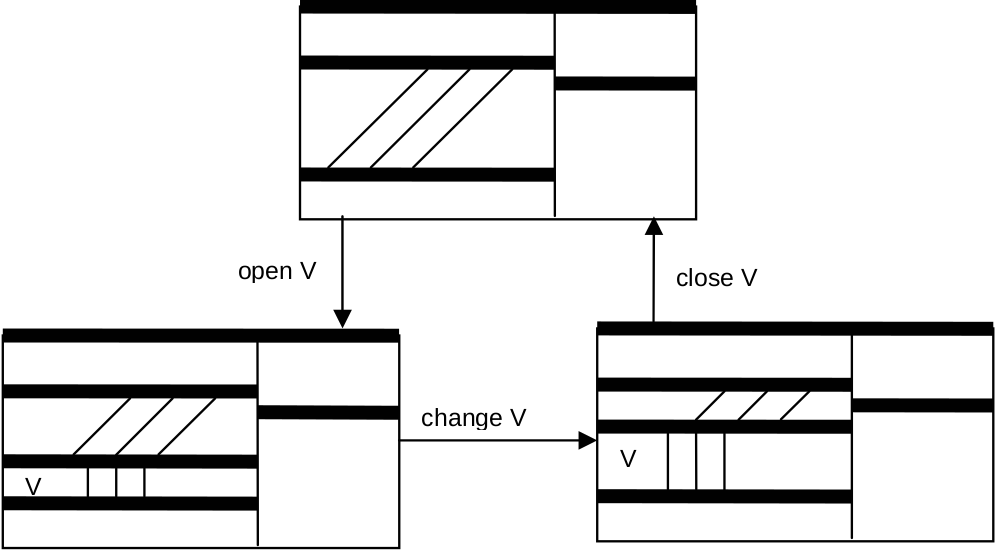
\includegraphics[width=.75\textwidth]{i/8}
  \caption{Basic operations on viewers}
  \label{fig:operation}
\end{figure}

The last group provides miscellaneous services.
\begin{itemize}
  \item \verb|This| identifies the viewer displayed at \verb|(X, Y)|.
  \item \verb|Next| returns the next upper neighbor of a given displayed viewer \verb|V|.
  \item \verb|Recall| allows recalling and restoring the most recently closed viewer.
  \item \verb|Locate| assists heuristic allocation of new viewers.
    For any given track and desired minimum height, it offers a choice
    of some distinguished viewers in this track:
    \begin{itemize}
      \item the \verb|fil|\textcolor{gray}{ler} viewer,
      \item the one at \verb|bot|\textcolor{gray}{tom},
      \item an \verb|alt|\textcolor{gray}{ernative} choice, and
      \item the viewer of \verb|max|\textcolor{gray}{imum} height.
    \end{itemize}
  \item Finally, \verb|Broadcast| broadcasts a message to the display area, that is,
    sends the given message to all currently displayed viewers.
\end{itemize}

It is now a good time to throw a glance behind the scenes.
Let us start with revealing \verb|Viewer| internal data structure.
Remember that according to the principle of information hiding
an internal data structure is fully private to the containing module
and accessible only through the module’s procedural interface.  Fig \ref{fig:snapshot}
shows a data structure view of the display snapshot taken in Fig \ref{fig:overlay}.
Note that the overlaid tracks and viewers are still part of the internal data structure.
\begin{figure}[h!]
  \centering
  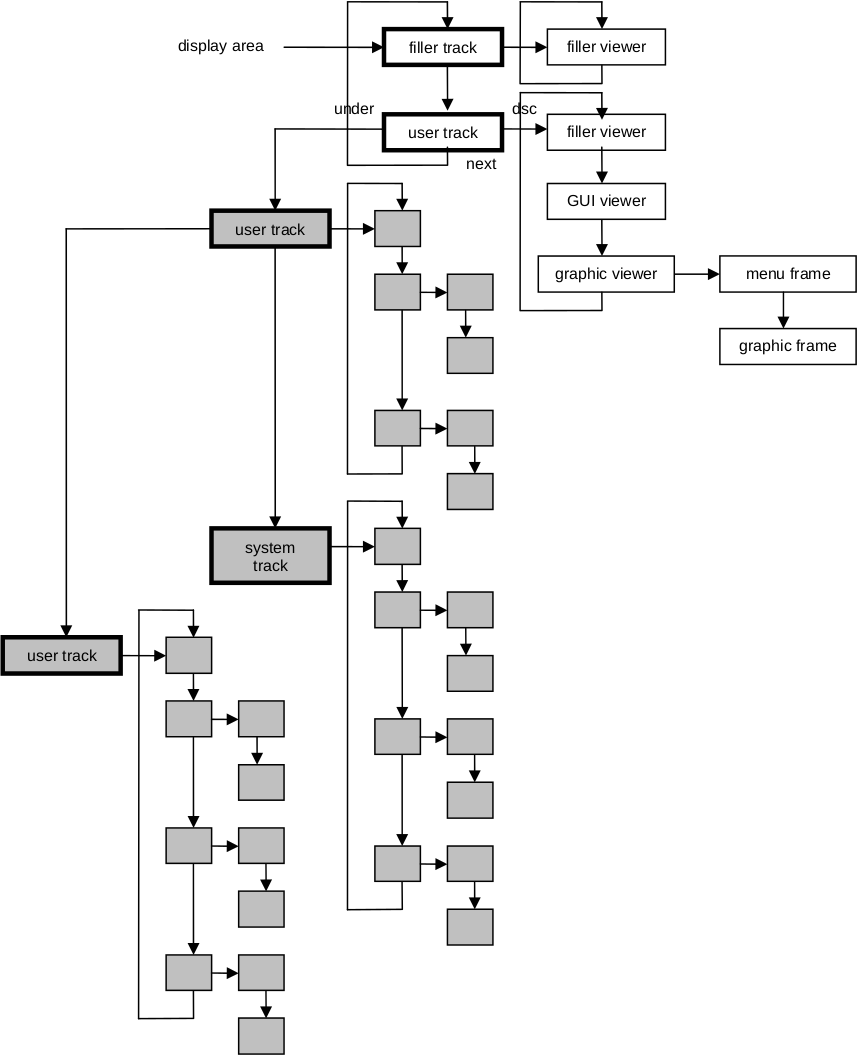
\includegraphics[width=\textwidth]{i/9}
  \caption{Internal data structure snapshot of Fig \ref{fig:overlay}}
  \label{fig:snapshot}
\end{figure}

In the data structure we recognize an anchor that represents the display area
and points to a list of tracks, each track pointing to a list of viewers,
each viewer in turn pointing to a list of arbitrary sub-frames.
Both the list of tracks and the list of viewers are closed to a ring,
where the filler track (filling up the display area)
and the filler viewers (filling up the tracks) act as anchors.
Additionally, each track points to a (possibly empty) list of tracks lying underneath.
These frames are invisible on the display, and shaded in Fig \ref{fig:snapshot}.

Technically, the track descriptor \verb|TrackDesc| is a private extension
of the viewer descriptor \verb|ViewerDesc|.
Repeating the declarations of viewer descriptors and frame descriptors,
we get to this hierarchy of types:
\begin{verbatim}
   TrackDesc = RECORD (ViewerDesc)
                      under: Display.Frame   END;

  ViewerDesc = RECORD (FrameDesc) state: INT END;

   FrameDesc = RECORD  next, dsc: Frame;
                      X, Y, W, H: INT;
                          handle: Handler    END;
\end{verbatim}

It is noteworthy that the data structure of the VM is heterogeneous with \verb|Frame| as base type.
It provides a nice example of a nested hierarchy of frames with the additional property
that the 1st 2 levels correspond to the 1st 2 levels in the type hierarchy defined by
\verb|Track|, \verb|Viewer|, and \verb|Frame|.

In an object-oriented environment objects are autonomous entities in principle.  However,
they may be bound to some higher instance (other than the system) temporarily.  For example,
we can look at the objects belonging to a module's private data structure as bound to this module.
Deciding if an object is currently bound then becomes a fundamental problem.  In the case of viewers,
this information is contained in an extra instance variable called \verb|state|.

As a system invariant, we have for every viewer $V$
\[ V\text{ is bound to module }Viewers \Leftrightarrow V.state \neq 0 \]
If we call any displayed viewer \emph{visible} and
each covered by an overlaying track \emph{suspended}, we can refine this invariant to
\begin{align*}
\{V\text{ is }&  visible\!\!\!\!\!\!\!\!\!\!\!\!\!\!\!\!\!\!\!\!\!\!\!\!\!\!\!&\Leftrightarrow V.state > 0\}&\text{ and }\\
\{V\text{ is }&suspended\!\!\!\!\!\!\!\!\!\!\!\!\!\!\!\!\!\!\!\!\!\!\!\!\!\!\!&\Leftrightarrow V.state < 0\}&
\end{align*}
In addition,
more detailed information about the kind of viewer $V$ is given by the magnitude $|V.state|$:
\begin{table}[h!]
  \centering
  \begin{tabular}{r l}
    $|V.state|$ & kind of viewer \\\hline
              0 & closed \\
              1 & filler \\
             -1 & productive
  \end{tabular}
\end{table}
\\The magnitude $|V.state|$ is kept invariant by \verb|Viewers|.
It could be used, for example, to distinguish different levels of importance or preference
with the aim of supporting a smarter algorithm for heuristic new viewers allocation.
$state$ is read-only to modules other than \verb|Viewers|.

We are now sufficiently prepared to understand how the exported \verb|Viewers| procedures
work behind.  They all operate on the internal dynamic data structure just explained.
\begin{itemize}
  \item \verb|This|, \verb|Next|, \verb|Locate|, \verb|Change| use it as a reference only
    or operate on individual elements
  \item \verb|InitTrack|, \verb|OpenTrack|, \verb|Open| add new elements, and
  \item \verb|CloseTrack|, \verb|Close| remove elements.
\end{itemize}
Most have side-effects on existing elements ($size$ or $state$).

Let us now change perspective and look at \verb|Viewers| as
a general low-level viewer manager (VMer) whose exact contents are unknown to it
(and whose controlling software might have been developed years later).
In short, let us look at \verb|Viewers| as a manager of black boxes.
Such an abstraction immediately makes it impossible for the implementation to call fixed procedures
for, say, changing a viewer's size or state.
The facility needed is a \emph{message-oriented interface}.
\begin{verbatim}
  TYPE ViewerMsg = RECORD (Display.FrameMsg) id,
                          X, Y, W, H, state: INT END;
\end{verbatim}

There're 3 variants of \verb|Viewer| messages, discriminated by \verb|id|:
\begin{table}[h!]
  \centering
  \begin{tabular}{l}
    restore contents, \\
    modify height (extend or reduce at bottom), and \\
    suspend (close temporarily or permanently).
  \end{tabular}
\end{table}
\\The additional components of the message inform about the desired new location, size, and state.
The following table lists senders, messages, and recipients of viewer messages.
\begin{table}[h!]
  \setlength{\tabcolsep}{1pt}
  \begin{tabular}{l|l|c r}
    \small{Originator} & \multicolumn{1}{c}{Message} & \multicolumn{2}{|c}{Recipients} \\\hline
    \small{OpenTrack}  & \small{suspend temporarily}
                       & \multicolumn{2}{l}{\small{viewers covered by opening track}} \\
    \small{CloseTrack} & \small{suspend permanently}
                       & \multicolumn{2}{l}{\small{viewers in closing track}}         \\
    \small{Open}       & \small{modify or suspend}
                       &        upper        &  opening viewer \\
    \small{Change}     & \small{modify}
                       & \small{neighbor of} & changing viewer \\
    \small{Close}      & \small{suspend permanently} & \multicolumn{2}{r}{closing viewer}
  \end{tabular}
\end{table}

\subsection{Menu Viewers}
\label{sub:menuviewers}
So far, we have treated viewers abstractly.
Next step we focus on a special class called \emph{menu viewers}.
From the earlier definition we know they're characterized by a structure
consisting of 2 vertically tiled \emph{descendant} frames,
\begin{table}[h!]
  \centering
  \begin{tabular}{r l}
    a frame of & at the \\\hline
    menu       & top, and \\
    contents   & bottom.
  \end{tabular}
\end{table}
\\Because the nature and contents of these frames are typically unknown
by their “ancestor” (or “parent”) viewer,
a collection of abstract messages is again a postulating form of interface.
As net effect, the handling of menu viewers boils down to a combination
of preprocessing, transforming and forwarding messages to the descendant frames.
In short, the display space is hierarchically organized and message passing within it
obeys the pattern of strict parental control.

Again, we start detailed discussion with module interface:
\begin{verbatim}
  DEFINITION MenuViewers;
    IMPORT Viewers, Display;        (*message ids*)
    CONST extend = 0; reduce = 1; move = 2;
    TYPE Viewer = POINTER TO ViewerDesc;
         ViewerDesc = RECORD (Viewers.ViewerDesc)
                             menuH: INT        END;
         ModifyMsg = RECORD (Display.FrameMsg)
                            id, dY, Y, H: INT  END;
  
    PROC Handle(       V: Display.Frame;
                   VAR M: Display.FrameMsg);

    PROC New(Menu , Main: Display.Frame;
             menuH, X, Y: INT             ): Viewer;
  END MenuViewers.
\end{verbatim}
The interface represented by this definition is conspicuously narrow.
There are just 2 procedures:
\begin{itemize}
  \item[a] generator procedure \verb|New|, and

    Returns a newly created menu viewer displaying the 2 (arbitrary) frames passed as parameters.

  \item[a] standard message handler \verb|Handle|.

    Implements the entire “behavior” of an object and in particular
    the above message dispatching functionality.
\end{itemize}

Message handlers in Oberon are implemented in the form of procedure variables that obviously
must be initialized properly at object creation time.  In other words, some concrete behavior
must explicitly be bound to each object, where different instances of the same object type
could potentially have a different behavior and/or the same instance could change its behavior
during its lifetime.  Our object model is therefore \emph{instance-centered}.

Conceptually, the creation of an object is an atomic action consisting of 3 basic steps:
\begin{enumerate}
  \item Allocate memory block;
  \item Install message handler;
  \item Initialize state variables.
\end{enumerate}
In the case of a standard menu \verb|V|\textcolor{gray}{iewer} creation:
\begin{verbatim}
  NEW(V); V.handle := Handle; V.dsc      := Menu;
          V.menuH  := menuH ; V.dsc.next := Main
\end{verbatim}
\verb|New| equals to \verb|create V; open V at X,Y|.
Opening \verb|V| needs \verb|Viewers|' assistance.

Implementing \verb|Handle| embodies the standard message handling strategy.
This is a coarse-grained view:
\begin{verbatim}
IF message reports about user interaction THEN
  IF variant is mouse tracking THEN
    IF mouse is in menu region THEN
      IF mouse is in upper menu region and
         left key is pressed THEN
        handle changing of viewer
      ELSE delegate handling to menu-frame
      END
    ELSE
      IF mouse is in main-frame THEN
        delegate handling to main-frame
      END
    END
  ELSIF variant is keyboard input THEN
    delegate handling to menu frame;
    delegate handling to main frame
  END

ELSIF message defines generic operation THEN
  IF message requests copy (clone) THEN
    send copy-message to menu frame to get a copy;
    send copy-message to main frame to get a copy;
    create menu viewer clone from copies
  ELSE
    delegate handling to menu frame;
    delegate handling to main frame
  END

ELSIF message reports about change of contents THEN
  delegate handling to menu frame;
  delegate handling to main frame

ELSIF message requests change of location/size THEN
  IF operation is restore THEN
    draw viewer area and border;
    send menu frm modify-msg to make extend from H 0;
    send main frm modify-msg to make extend from H 0
  ELSIF operation is modify THEN
    IF operation is extend THEN
      extend viewer area and border;
      send modify-msg to menu frm to make it extend;
      send modify-msg to main frm to make it extend
    ELSE (*reduce*)
      send modify-msg to main frm to make it reduce;
      send modify-msg to menu frm to make it reduce;
      reduce viewer area and border
    END
  ELSIF operation is suspend THEN
    send main frm modify-msg to make reduce to H 0;
    send menu frm modify-msg to make reduce to H 0
  END
END
\end{verbatim}

In principle, the handler acts as a message dispatcher that either processes a message directly
and/or delegates its processing to the descendant frames. Note that the handler's main alternative
statement discriminates precisely among the 4 basic categories of messages.

From the above outlined algorithm, handling copy messages, that is, requests for generating
a copy or clone of a menu viewer, we can derive a general recursive scheme for the creation
of a clone of an arbitrary frame:
\begin{enumerate}
  \item Send copy message to each element in the list of descendants;
  \item Generate copy of the original frame descriptor;
  \item Attach copies of descendants to the copy of descriptor.
\end{enumerate}

The essential point here is the use of new outgoing messages
in order to process a given incoming message.
We can regard message processing as a transformation
mapping incoming messages into a set of outgoing ones, with possible side-effects.
The simplest one, the input message being simply passed on to descendant(s),
is called \emph{delegation}.

As a fine point we clarify that the above algorithm is designed to create a deep copy
of a composite object (a menu viewer in our case).  If a shallow copy would be desired,
the descendants would not have to be copied, and the original descendants
instead of their copies would be attached to the copy of the composite object.

Another example of message handling is provided by mouse tracking.  Assume that
a mouse message is received by a menu viewer while the mouse is located in the upper part
of its menu frame and the left mouse key is kept down.  This means "change viewer's height
by moving its top line vertically".  No message to express the required transformation
of the sub-frames yet exists.  Consequently, module \verb|MenuViewer|s takes advantage of
our open (extensible) message model and simply introduces one called:
\begin{verbatim}
  ModifyMsg = RECORD (Display.FrameMsg)
                id, dY, Y, H: INT
              END;
\end{verbatim}
Field \verb|id| specifies one of the following 2 variants:
\begin{enumerate}
  \item \emph{extend}, or

    Requests the frame to move by the vertical translation vector \verb|dY|
    and then extend to height \verb|H| at bottom.

  \item \emph{reduce}.

    Requests the frame to reduce to height \verb|H| at bottom
    and then move by \verb|dY|.
\end{enumerate}
In both cases \verb|Y| indicates the Y-coordinate of the new lower-left corner.
Fig \ref{fig:modify} summarizes this graphically.
\begin{figure}[h!]
  \centering
  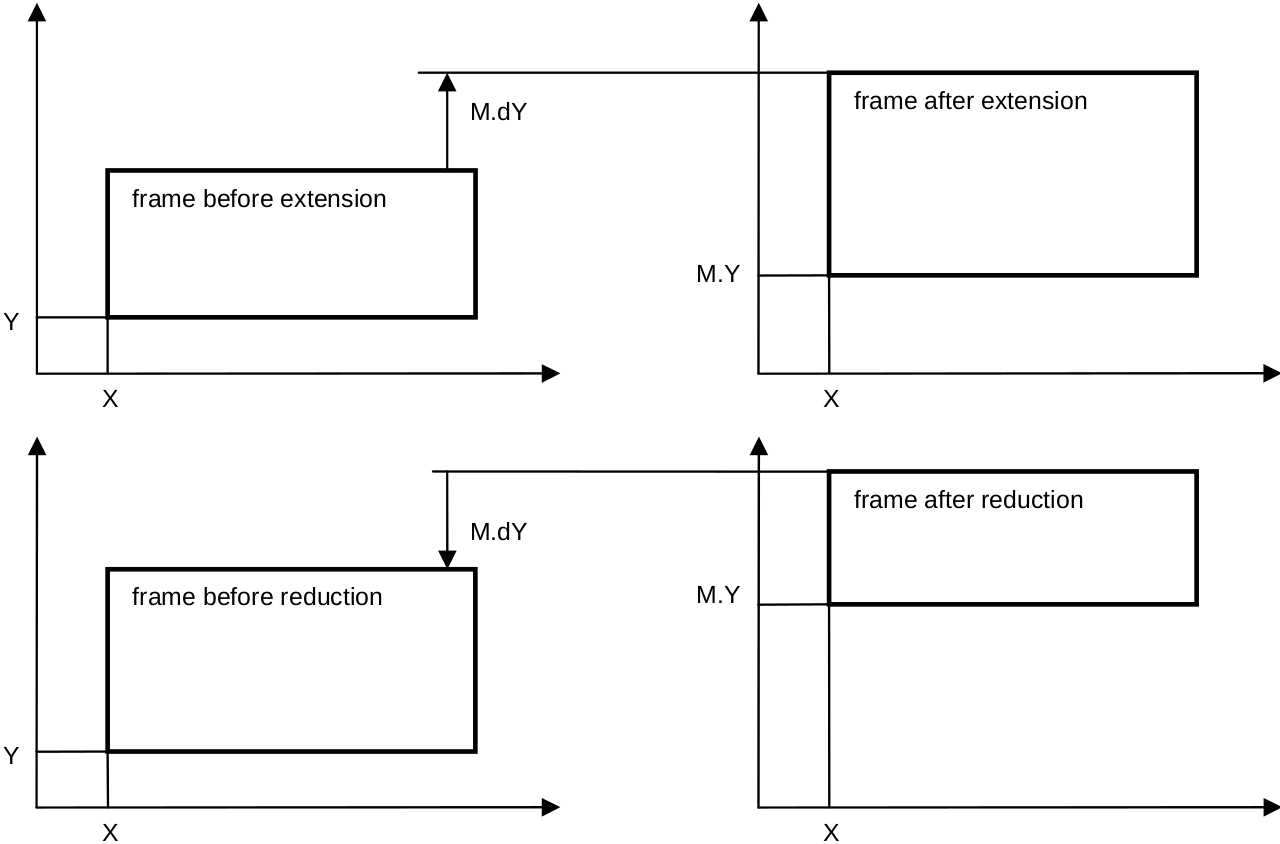
\includegraphics[width=.9\textwidth]{i/a}
  \caption{The modify frame operation}
  \label{fig:modify}
\end{figure}

Messages arriving from the VMer requesting the receiving viewer to extend or reduce
at its bottom are also mapped into \verb|ModifyMsg|s. Of course, no translation, $dY = 0$.

The attentive reader might perhaps have asked why the standard handler
is exported by \verb|MenuViewers| at all.  The thought behind is code reusability.
For example, a message handler for a subclass of menu viewers could be implemented effectively
by reusing menu viewer's standard one.  After having first handled all new or differing cases
it would simply (super-)call the standard handler subsequently.

\subsection{Cursor Management}
Traditionally, a cursor indicates and visualizes on the screen the current location of the caret
in a text or, more generally, the current \emph{focus of attention}.
A small arrow or similar graphic symbol is typically used for this purpose.
In Oberon, we have slightly generalized and abstracted this concept.
A cursor is a path in the logical display area whose current position can be made visible by a \emph{marker}.

The VMer and the cursor handler are 2 concurrent users of the same display area.
Actually, we should imagine 2 parallel planes,
\begin{table}[h!]
  \centering
  \begin{tabular}{r l}
              & displaying \\\hline
          one & viewers, and \\
    the other & cursors.
  \end{tabular}
\end{table}
\\If there's just 1 physical plane we take care of painting markers non-destructively, for example
in inverse-video mode.  Then, no precondition must be established before drawing a marker.
However, in the case of a viewer task painting destructively in its viewer's area,
the area must be locked first after turning invisible all markers in the area.

The technical support of cursor management is also contained in \verb|Oberon|.
The corresponding API:
\begin{verbatim}
DEFINITION Oberon;
  TYPE Marker = RECORD Fade,Draw: PROC(x,y: INT) END;
       Cursor = RECORD marker: Marker; X,Y: INT;
                                        on: BOOL END;
  VAR Arrow, Star   : Marker;
      Mouse, Pointer: Cursor;

  PROC OpenCursor(VAR c: Cursor);
  PROC FadeCursor(VAR c: Cursor);
  PROC DrawCursor(VAR c: Cursor;
                  VAR m: Marker; X, Y: INT);
  PROC MarkedViewer(): Viewers.Viewer;
  PROC RemoveMarks(X, Y, W, H: INT);
  ...
END Oberon.
\end{verbatim}
The state of a cursor is given by
\begin{table}[h!]
  \centering
  \begin{tabular}{r l}
    \verb|on|     & its mode of visibility, \\
    \verb|(X, Y)| & its position in the display area, and \\
    \verb|marker| & the current marker.
  \end{tabular}
\end{table}
\\\verb|Marker| is an abstract data type with an interface consisting of operations
  \verb|Fade| and
  \verb|Draw|.
The main benefit of this abstraction is once more conceptual independence
of the underlying hardware.  For example, they can
\begin{itemize}
  \item adapt to a given monitor hardware with built-in cursor support or,
    in case of absence of such support, simply
  \item be implemented as identical procedures (an involution)
    drawing the marker pattern in inverse video mode.
\end{itemize}

The functional interface to cursors consists of 3 operations:
\begin{table}[h!]
  \centering
  \begin{tabular}{l l}
    ~-\verb|Cursor| & to \\\hline
    \verb|Open| & open a new cursor, \\
    \verb|Fade| & switch off the marker of an open cursor, and \\
    \verb|Draw| & extend the path of a cursor to a new position \\
                & and mark it with the given marker.
  \end{tabular}
\end{table}
\\We emphasize that
the marker representing a given cursor can change its shape dynamically on the fly.

2 cursors are predefined:
\begin{table}[h!]
  \centering
  \begin{tabular}{r c l}
    cursor         & represents & \small{built-in }marker\small{ typically} \\\hline
    \verb|Mouse|   & the mouse  & \small{a small NW-pointing }\verb|Arrow| \\
    \verb|Pointer| &  a global  & \small{a }\verb|Star|\small{ symbol} \\
                   & \small{system pointer}
  \end{tabular}
\end{table}
\\The pointer can be used to mark any displayed object.
It serves primarily as an implicit parameter of commands.

2 assisting service procedures are added in connection with the predefined cursors:
\begin{table}[h!]
  \setlength{\tabcolsep}{3pt}
  \begin{tabular}{l|l}
    \verb|Marked| & \small{returns the viewer currently marked by the pointer,} \\
    \verb|-Viewer|& \small{equivalent to \verb|Viewers.This(Pointer.X, Pointer.Y)|.} \\\hline
    \verb|Remove| & \small{turns invisible within a given rectangle in display area,} \\
    \verb|-Marks| & \small{used to lock the rectangle for its caller.}
  \end{tabular}
\end{table}

Summary the essential concept points of cursor handling:
\begin{itemize}
  \item By virtue of the use of
    \begin{itemize}
      \item abstract markers, and
      \item the logical display area,
    \end{itemize}
    any potential hardware dependence is encapsulated in system modules
    and is therefore hidden from the application programmer.
    Cursors are moving uniformly within the whole display area,
    even across screen boundaries.

  \item Cursor handling is decentralized by delegating it to the individual handlers
    that are installed in viewers.  Typically, a handler reacts on the receipt
    of a mouse tracking message by drawing the mouse cursor at the indicated new position.
    The benefit of such individualized handling is flexibility.  For example,
    a smart local handler might choose the shape of the visualizing marker
    depending on the exact location, or it might force the cursor onto a grid point.

  \item Even though cursor handling is decentralized, there is some intrinsic support
    for cursor drawing built into the \verb|Cursor| declaration.
    Cursors are full value objects and, as such, can "memorize" their current state.
    Consequently, the interface operations \verb|FadeCursor| and \verb|DrawCursor|
    need to refer to the desired future state only.

  \item Looking at the VMer as one user of the display area, the cursor handler
    is the 2nd (and logically concurrent) user of the same resource.  If there is
    just one physical plane implementing the display area, any region must be locked
    by a current user before destructive painting.  Therefore,
    markers are usually painted non-destructively in inverse-video mode.
\end{itemize}

Let us now recapitulate the entire section.
\begin{itemize}
  \item The central resource managed by the display subsystem is the \emph{logical display area}
    whose purpose is abstraction from the underlying display monitor hardware.

    The display area is primarily used by the VMer for the accommodation of tracks and viewers,
    which are merely the 1st 2 levels of a potentially unlimited nested hierarchy of display frames.
    For example, standard menu viewers contain 2 subordinate frames:
    \begin{itemize}
      \item a menu frame, and
      \item a main frame of contents.
    \end{itemize}

  \item Viewers are treated as black boxes by the VMer and are addressed via messages.

    Viewers and, more generally frames, are used as elements of \emph{message-based interfaces}
    connecting the display subsystem with other subsystems like
    \begin{itemize}
      \item the task scheduler, and
      \item the various document managers.
    \end{itemize}

  \item Finally, the display area is also the living room of cursors.  In Oberon,
    a cursor is a marked path, 2 standard cursors \verb|Mouse| and \verb|Pointer| are predefined.
\end{itemize}
